% !TEX root =  ../main.tex

\begin{figure*}[t]
	\centering
	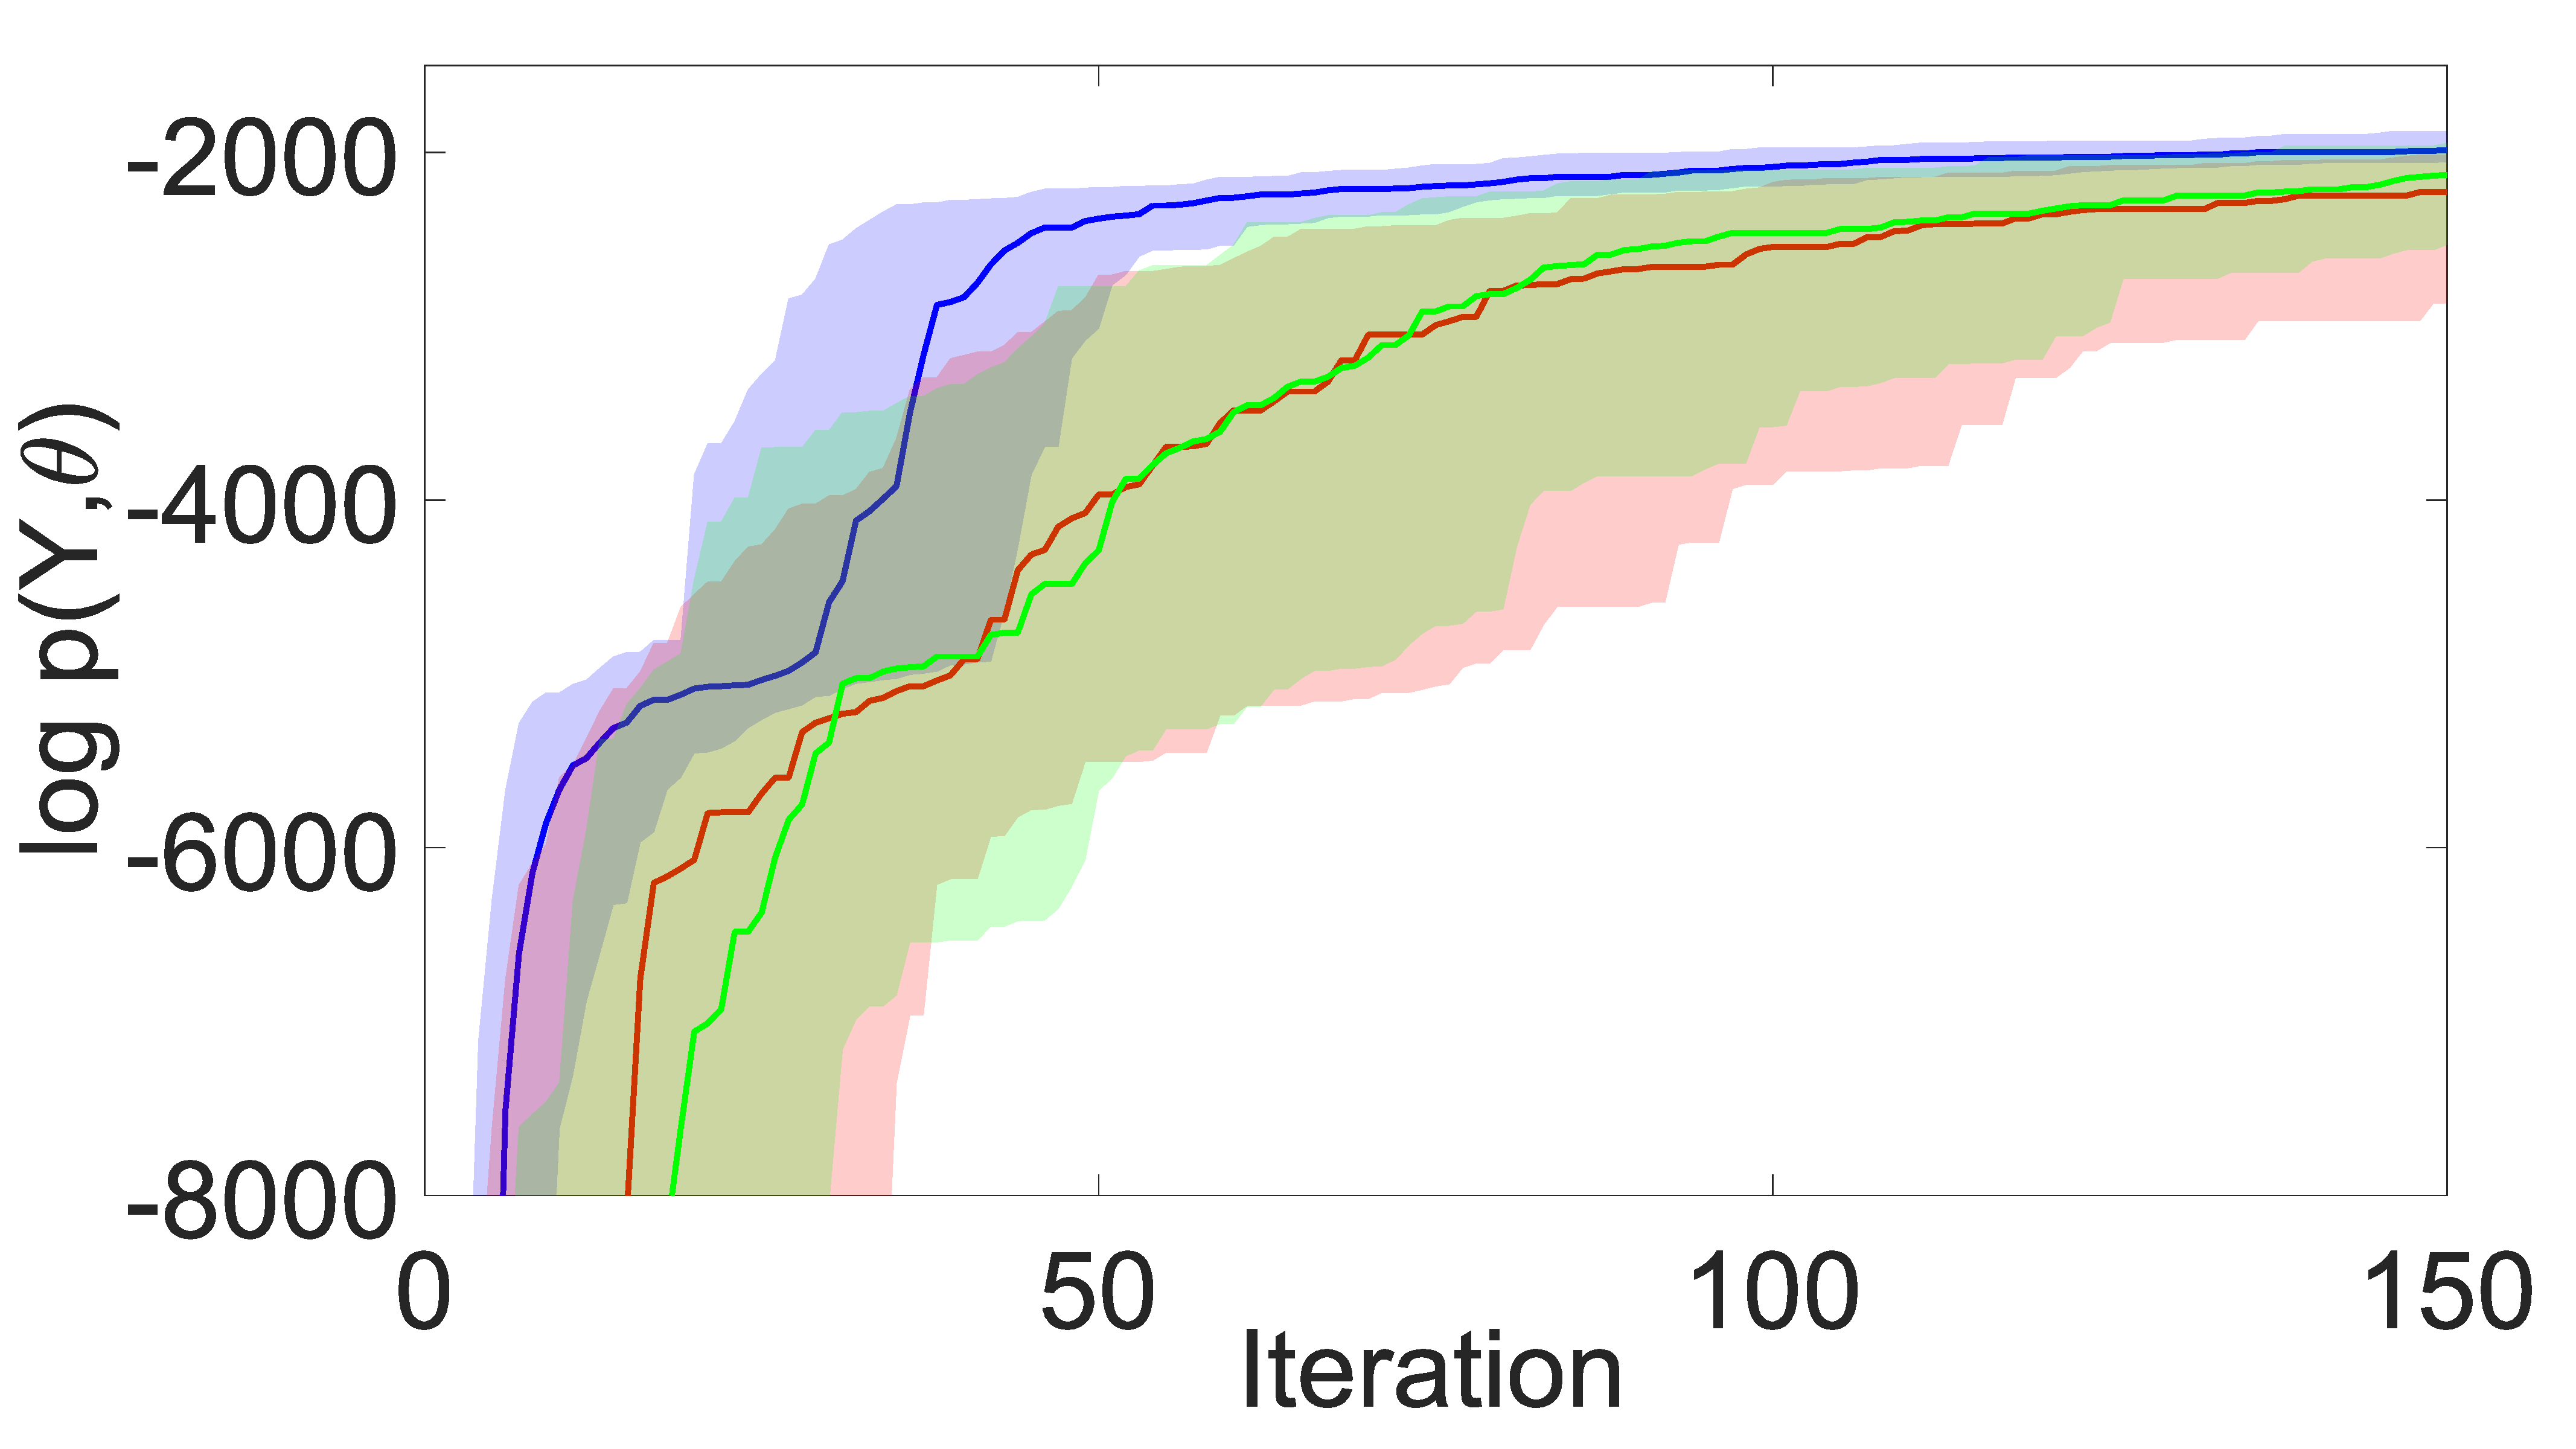
\includegraphics[width=2.72in]{hmm/hmm_ML}
	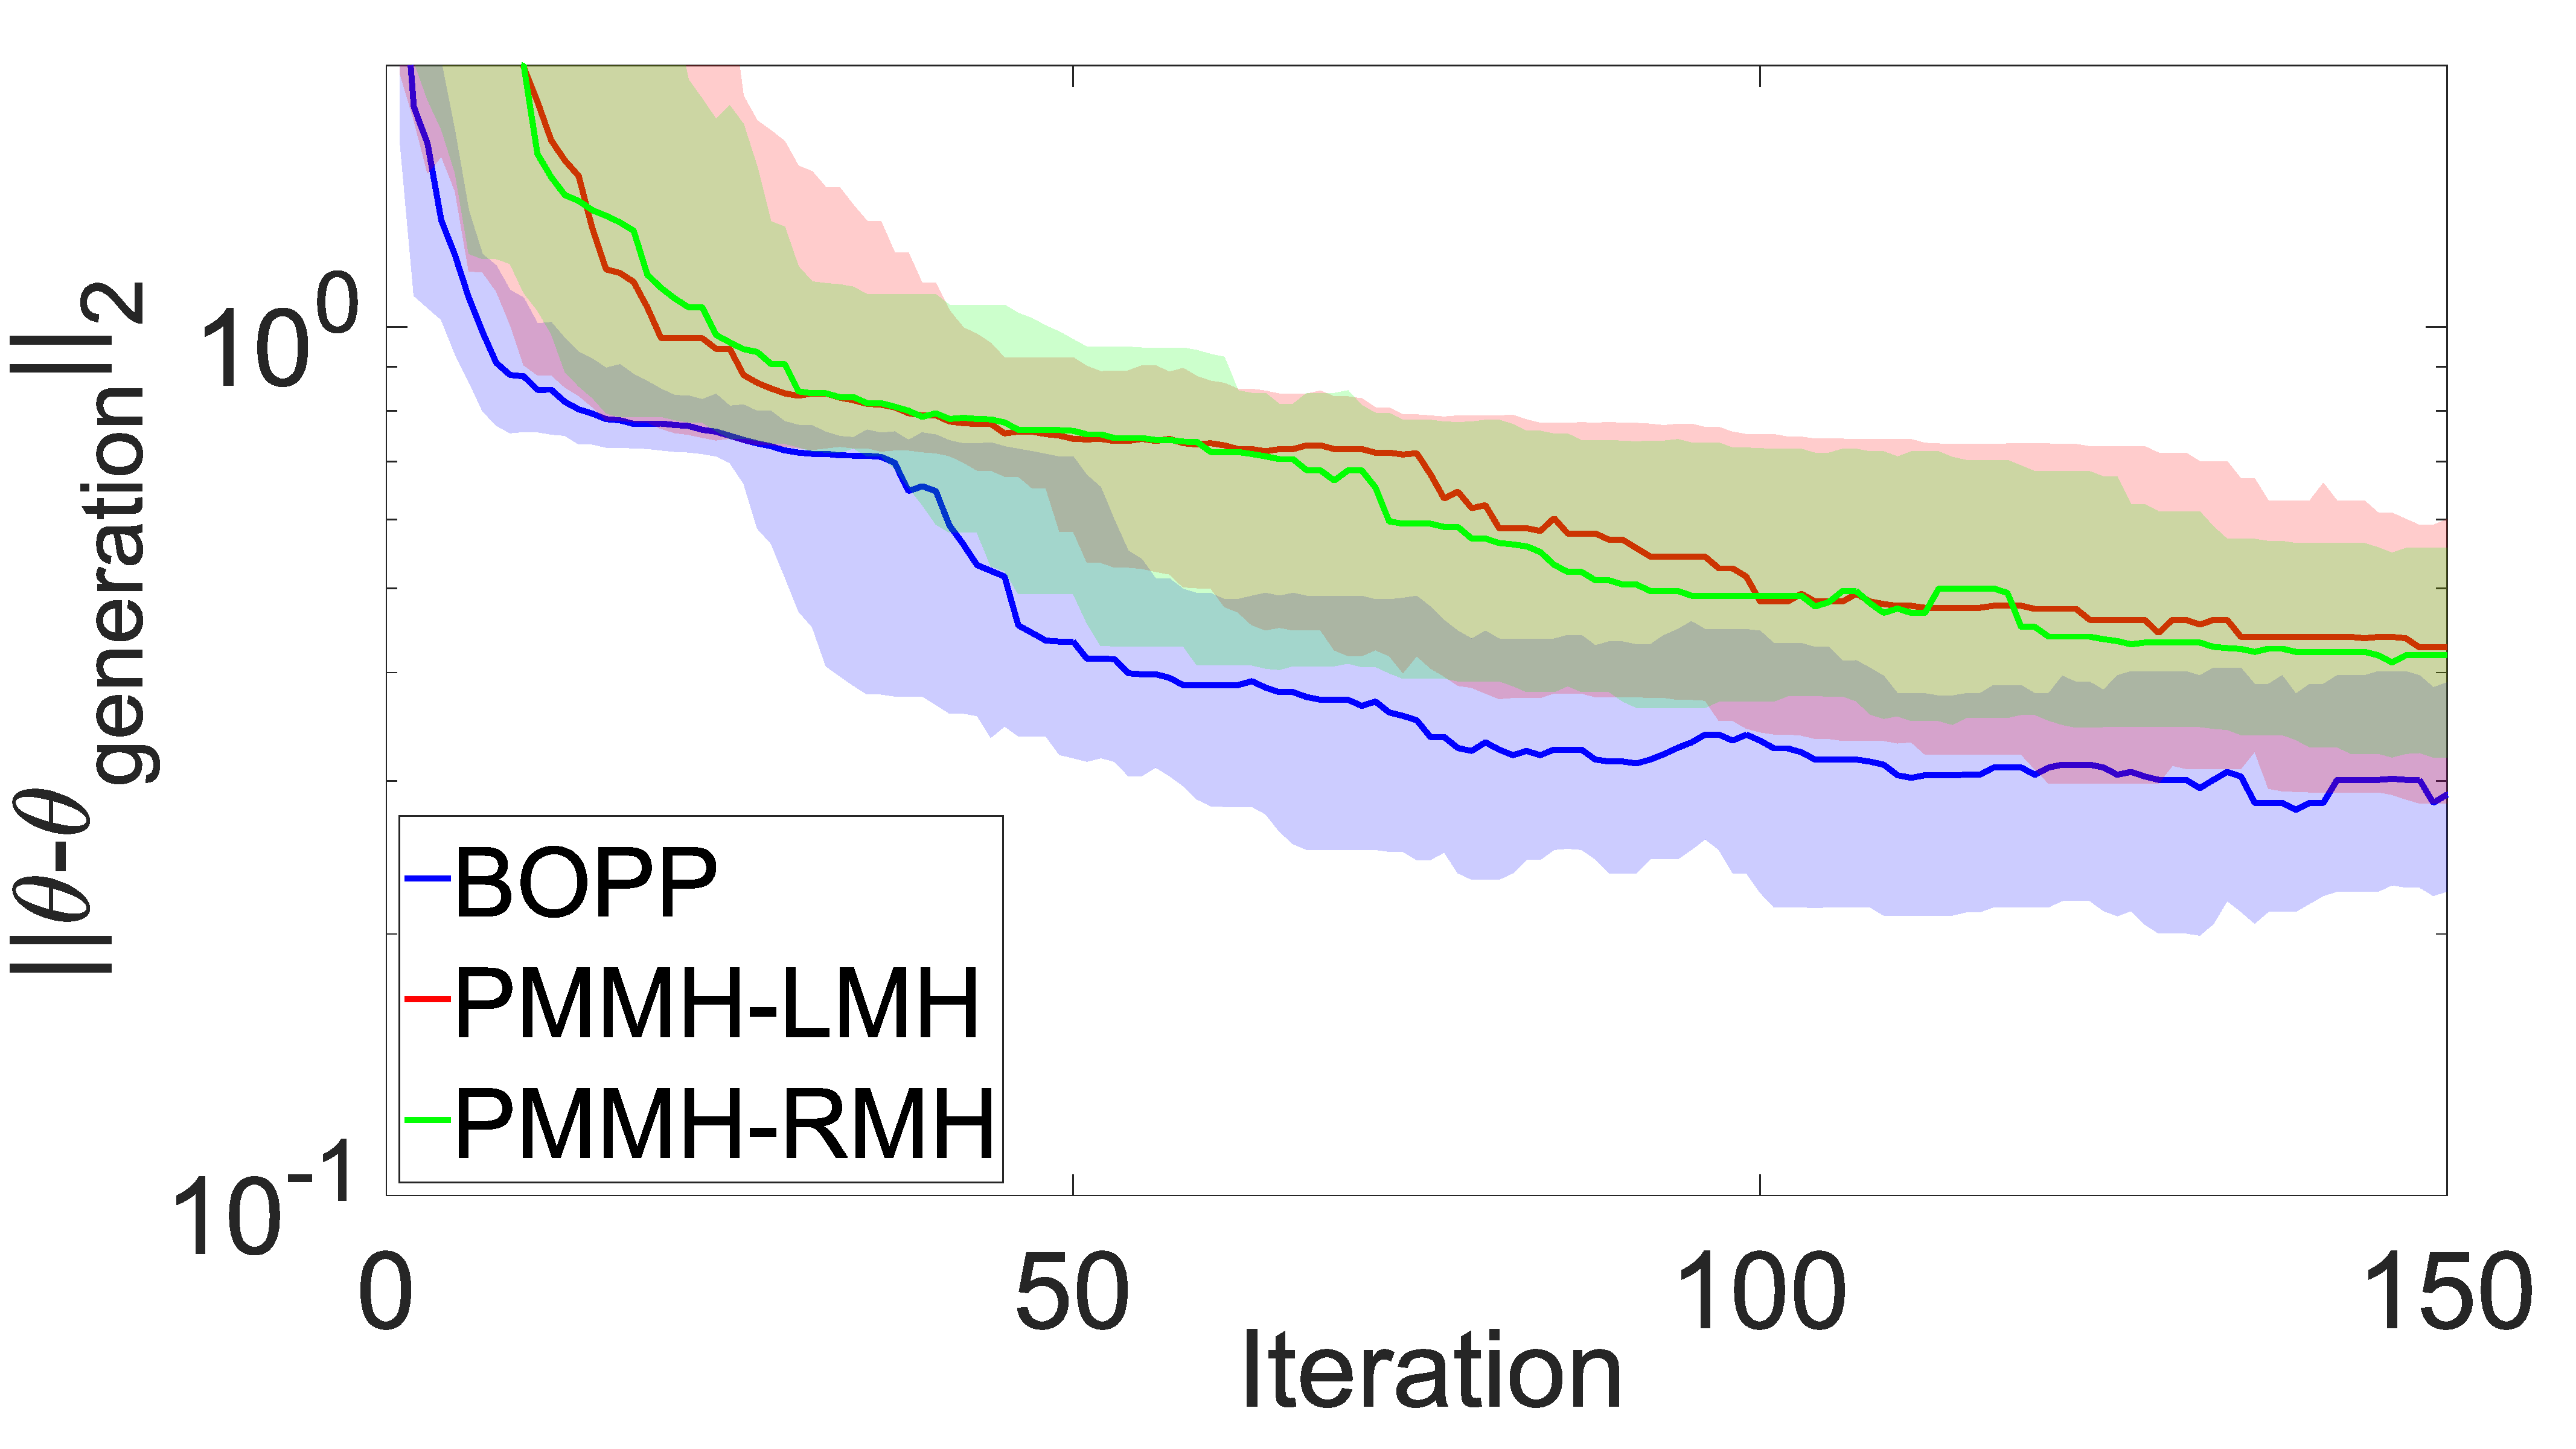
\includegraphics[width=2.72in]{hmm/hmm_distance}
	\caption{Convergence for HMM in terms of the cumulative best $\log p\left(Y,\theta\right)$ (\emph{left}) and distance to the ``true" $\theta$ used in generating the data (\emph{right}). Solid line shows median over 100 runs, whilst the shaded region the 25/75\% quantiles.  Note that for the distance to true $\theta$ was calculated by selecting which three states (out of the 5 generates) that were closest to the true parameters.  \label{fig:hmm}}
\end{figure*}

We finally consider a hidden Markov model (HMM) with an unknown number of states.  This example demonstrates how BOPP can be applied to models which conceptually have an unknown number of variables, by generating all possible variables that might be needed, but then leaving some variables unused for some execution traces.  This avoids problems of varying base measures so that the MMAP problem is well defined  and provides a function with a fixed number of inputs as required by the BO scheme.  From the BO perspective, the target function is simply constant for variations in an unused variable.

HMMs are Markovian state space models with discrete latent variables.  Each latent state $x_t \in\{1,\dots,K\}, t=1,\dots,T$ is defined conditionally on $x_{t-1}$ through a set of discrete transition probabilities, whilst each output $y_t\in\real$ is considered to be generated i.i.d. given $x_t$.  We consider the following HMM, in which the number of states $K$, is also a random variable: 
\begin{align}
\label{eq:hmm}
K & \sim \text{Discrete}\{1,2,3,4,5\} \\\displaybreak[0]
T_k &\sim \text{Dirichlet}\{{1}_{1:K}\}, \quad \forall k=1,\dots,K \\\displaybreak[0]
\phi_k &\sim \text{Uniform}[0,1], \quad \forall k=1,\dots,K \\\displaybreak[0]
\mu_0 &\leftarrow \min \{y_{1:T}\} \\\displaybreak[0]
\mu_k &\leftarrow \mu_{k-1}+\phi_k \cdot (\max \{y_{1:T}\} -\mu_{k-1}), \quad \forall k=1,\dots,K \\\displaybreak[0]
x_1 &\leftarrow 1 \\\displaybreak[0]
x_t | x_{t-1} &\sim \text{Discrete}\{T_{x_{t-1}}\}\\\displaybreak[0]
y_t | x_t &\sim\mathcal{N}(\mu(x_{t-1}),0.2).
\end{align}
Our experiment is based on applying BOPP to the above model to do MMAP estimation with a single synthetic dataset, generated using $K=3, \;\mu_1 = -1, \;\mu_2 = 0, \;\mu_3 = 4, \;T_1 = [0.9,0.1,0], \;T_2=[0.2,0.75,0.05]$ and $T_3=[0.1,0.2,0.7]$.  

We use BOPP to optimize both the number of states $K$ and the stick-breaking parameters $\phi_k$, with full inference performed on the other parameters.  BOPP therefore aims to maximize
\begin{align}
\label{eq:hmm-marginal}
p(K,\phi_{k=1:5}|y_{t=1:T}) = \iint p(K,\phi_{k=1:5},x_{t=1:T},T_{k=1:K}|y_{t=1:T}) \mathrm{d}x_{t=1:T} \mathrm{d}T_{k=1:K}.
\end{align}
As with the chaotic Kalman filter example, we compare to two PMMH variants using the same code transformations.  The results, given in Figure~\ref{fig:hmm}, again show that BOPP outperforms these PMMH alternatives.